\documentclass[english]{tktltiki}
\usepackage[pdftex]{graphicx}
\usepackage{subfigure}
\usepackage{url}
\begin{document}
%\doublespacing
%\singlespacing
\onehalfspacing

\title{Assignment 3: Interaction prototyping for a handheld device}
\author{P�ter Ivanics}
\date{\today}

\maketitle

\numberofpagesinformation{\numberofpages\ pages + \numberofappendixpages\ appendices}
\keywords{}

\mytableofcontents

\section{Introduction}
	This report is a summary of the process on prototyping a restaurant-finder mobile application. The report is rolled out as one of the assignment of the Human-Computer Interaction course and serves the purpose to gain hands-on experience with the course material. 
	
	The goal of this report and assignment is to gain hands-on experience with paper-based prototyping and storyboarding of a mobile application. As a case study, the design of a simple restaurant finder mobile application is given and is described in this report. The initial prototypes, proposals and storyboards are displayed and briefly described in the following chapter. Further, some conclusions are derived and future improvements are suggested. 
	
\section{Discussion}
	\subsection{Sketches}
	
	\begin{figure}[h] 
		\begin{center}
			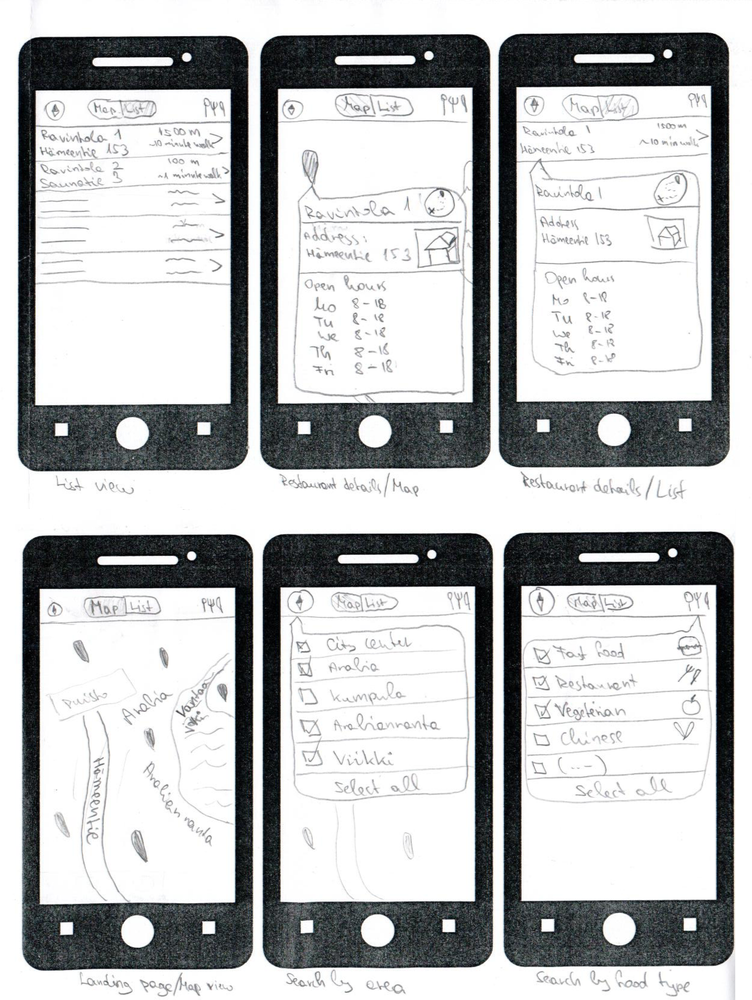
\includegraphics[width=0.8\textwidth]{images/sketch-1.png}
			\caption{Sketch 1 of the restaurant finder mobile application.}
			\label{sketch-1}
		\end{center}
	\end{figure}
	
	\begin{figure}[h] 
		\begin{center}
			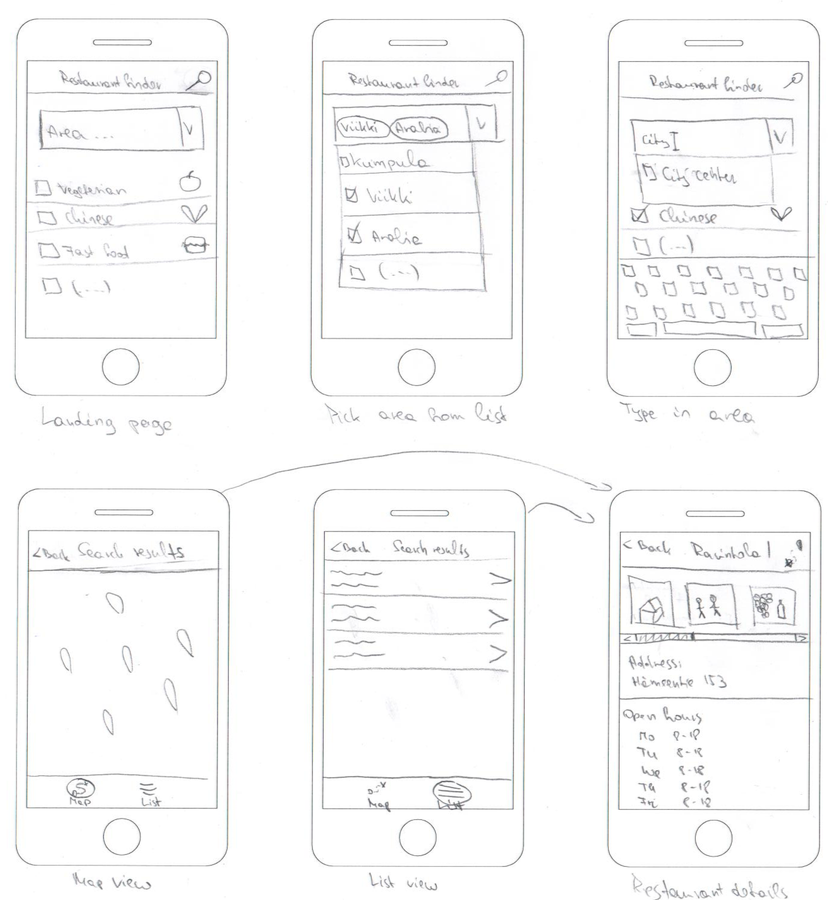
\includegraphics[width=0.8\textwidth]{images/sketch-2.png}
			\caption{Sketch 2 of the restaurant finder mobile application.}
			\label{sketch-1}
		\end{center}
	\end{figure}
	
	
	\subsection{Storyboards}
	
	
	\subsection{Prototype}

\section{Conclusions}
	
\pagebreak
\nocite{*}
\bibliographystyle{tktl}
\bibliography{bibliography}

\lastpage

\end{document}